\documentclass{article}
\usepackage{graphicx}
\usepackage{titlesec}
\usepackage{float}
\usepackage{fancyhdr}
\usepackage[english]{babel}
\usepackage[margin=2.2cm]{geometry}
\usepackage[utf8]{inputenc}
\usepackage[T1]{fontenc}
\usepackage{subcaption}
\usepackage{amsmath}

\graphicspath{{figures/}}

\titleformat*{\section}{\LARGE\bfseries}
\titleformat*{\subsection}{\large\bfseries}
\titleformat*{\subsubsection}{\small\bfseries}
 
\pagestyle{fancy}
\fancyhf{}
\rhead{Joachim Tapparel and Lennard Ludwig}
\lhead{Mini-project 2 : Framework}
\cfoot{\thepage}

\begin{document}
\thispagestyle{fancy}

\section{Framework}

Each module implements the following functions : 

\paragraph{forward(self, *input)}
The function computes the output from the given input and the parameters of the module.
    
\paragraph{backward(self, *gradwrtoutput)}
The function computes the derivative of the loss with respect to the input. In the case of a linear layer, in addition to the derivative, it accumulates the gradient of the loss with respect to its parameters. To compute it we can use the fact that trhe function takes as parameter the gradient of the loss with respect to the output and thus we have : 
\[\frac{\partial l}{\partial s} = \frac{\partial x}{\partial s} \frac{\partial l}{\partial x}\] 

where $\frac{\partial x}{\partial s}$ is the derivative of the forward function and $\frac{\partial l}{\partial x}$ is the derivative of the loss with respect to the output.

\paragraph{param(self)}
Returns a tuple of tenors containing the parameters of the model and their corresponding derivatives. 
    
\paragraph{reset(self)}
Resets the gradient accumulation of the linear layer to 0
    
\paragraph{update(self,eta)}
Updates the parameters of the module according to the gradient. The size of the step is given by the parameter eta defined by the user. 


In addition to the modules that define each layer, we added a module called \verb|Sequential| that contains all the modules of the network. It also has a function \verb|forward| and \verb|backward| that calls the forward/backward function for all its modules. This way when we want to use our framework we can simply add modules to our network and make steps ba simply calling \verb|forward| once. 
\\

The complete list of modules is the following:

\begin{itemize}
\item Activation layers:
 \begin{itemize}
	  \item ReLU
	  \item Tanh
	  \item Sigmoid
	  \end{itemize}
\item Linear Layer
\item Criterion :
 \begin{itemize}
	  \item Mean Absolute Error
	  \item Mean Square Error
	  \item Cross Entropy Loss
	  \end{itemize}
\end{itemize}

\subsection{Cross Entropy Loss}

In addition to the requested modules we decided to implement the cross entropy loss. Its forward expression is given by the following equation : 

\begin{equation}
\mathcal{L}(x) = - \log \left( \frac{e^{x_i}}{e^{x_i} + \Sigma_{n \ne i} e^{x_n}} \right) \text{where i is the target class} 
\end{equation}

From this expression we can compute the derivative with respect to x to compute the backward path. 
Before continuing we have to consider two cases, the one in which the input is part of the target class and the one in which the input isn't part of the target class.

\begin{equation}
\begin{array}{ll|l}
\frac{\partial}{\partial x_i} \mathcal{L}(x) & = \frac{\partial}{\partial x_i} \left( - \log \left( \frac{e^{x_i}}{e^{x_i} + \Sigma_{n \ne i} e^{x_n}} \right)\right) & \Sigma_{n \ne i} e^{x_n} = a\\
 & = \frac{\partial}{\partial x_i} \left( -\log(e^{x_i}) + \log(e^{x_i} + a) \right) & \\
 & = \frac{\partial}{\partial x_i} \left(-x_i\log(e) + \log(e^{x_i} + a) \right) &  \\
 & = - \frac{\partial}{\partial x_i} x_i + \frac{\partial}{\partial x_i}\log(e^{x_i} + a) & \\
 & = -1 + \frac{1}{e^{x_i} + a}e^{x_i} & \\
 & =  \frac{e^{x_i}}{\Sigma_{n} e^{x_n}} - 1 & 
\end{array}
\end{equation}

In a similar way we can calculate the second case : 

\begin{equation}
\begin{split}
\frac{\partial}{\partial x_j} \mathcal{L}(x) & = \frac{\partial}{\partial x_j} \left( - \log \left( \frac{e^{x_i}}{e^{x_j} + \Sigma_{n \ne j} e^{x_n}} \right)\right) \\
 & = \frac{e^{x_j}}{\Sigma_{n} e^{x_n}} \text{ as } \frac{\partial}{\partial x_j} x_i = 0
\end{split}
\end{equation}


We thus end up with an output that consists of the tensor :


\[\frac{\partial l}{\partial x} = \begin{pmatrix}
									\frac{\partial}{\partial x_1}\mathcal{L}(x) \\
									\frac{\partial}{\partial x_2}\mathcal{L}(x) \\
									\vdots \\
									\frac{\partial}{\partial x_n}\mathcal{L}(x) 
								  \end{pmatrix} \]
								  

\section{Test of the framework}

After building the requested network, we trained it on the random dataset. After several tests we got a test error of 7.71\% with a standard deviation of 0.0513

If we have a look at the graph of the test error versus the number of epochs we can observe that depending on the start weights, the error drops only after 50 epochs or later or even sometimes it gets stuck in a local minima.   

\begin{figure}[H]
\begin{center}
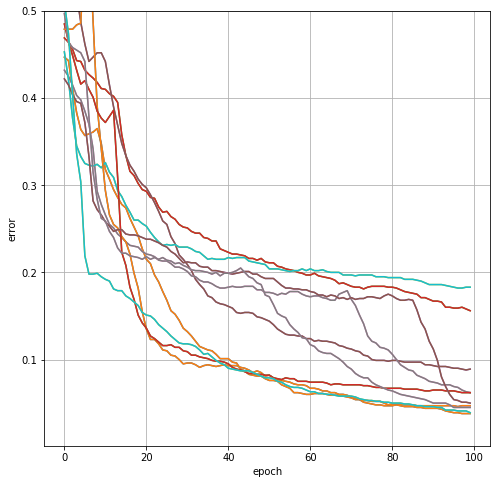
\includegraphics[width=0.47\textwidth]{err_mse_sep}
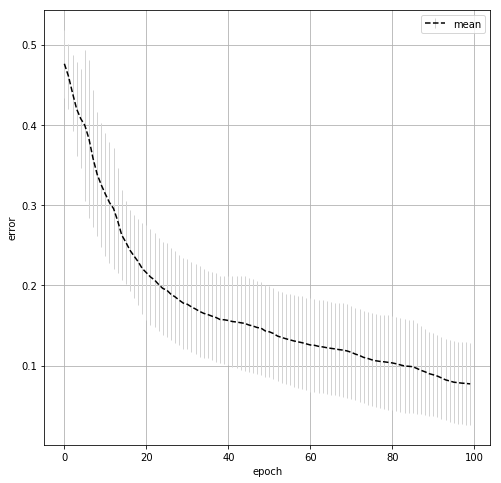
\includegraphics[width=0.47\textwidth]{err_mse}
\caption{Test error versus number of epochs}
\end{center}
\end{figure}

If we have a look at the classification of the output we get can see that the classified circle isn't exactly round but it works pretty good. 

\begin{figure}[H]
\begin{center}
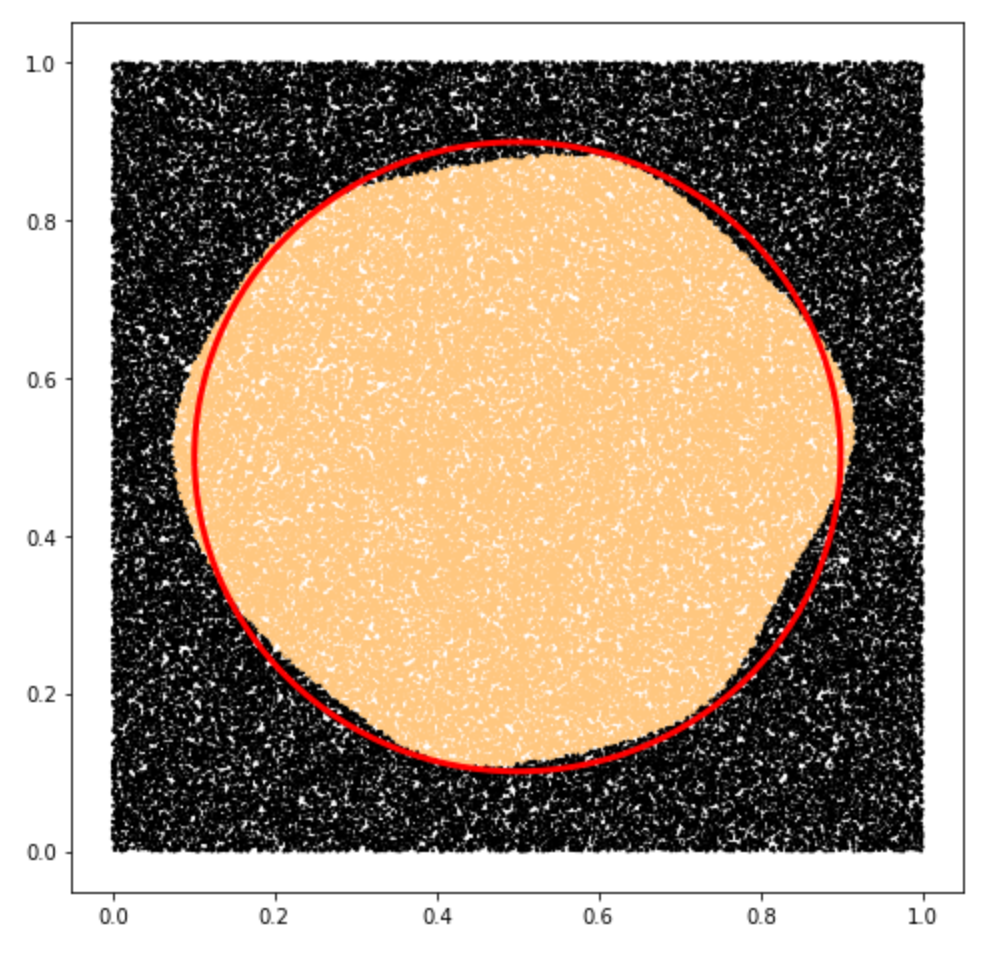
\includegraphics[width=0.5\textwidth]{mse_plot}
\caption{Output plot using MSE}
\end{center}
\end{figure}


We also tried with the Mean Absolute Error and the Cross Entropy Loss. We observed that MAE didn't work as well because it got stuck in local minima more often. With CEL we also achieved the best and most consistent results (minimal standard deviation of the error).
  
\begin{figure}[H]
\begin{center}
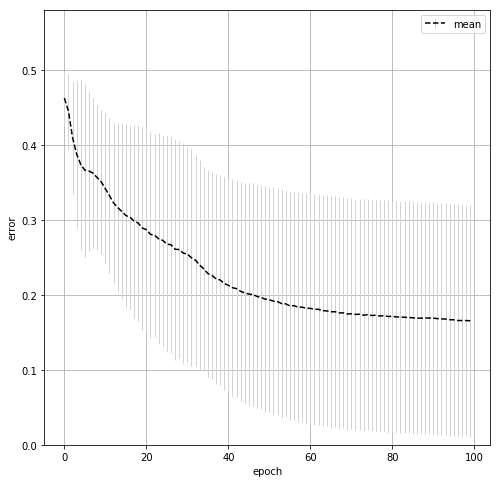
\includegraphics[width=0.47\textwidth]{err_mae}
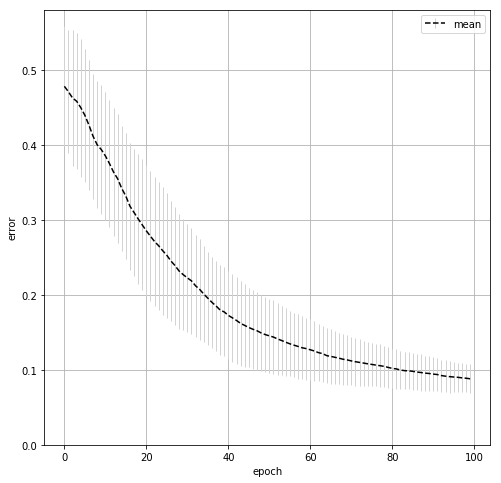
\includegraphics[width=0.47\textwidth]{cel_err}
\caption{Test error versus number of epochs for MAE and CEL respectively}
\end{center}
\end{figure}




\end{document}

%
%
%
%
%
%
%
%
%
%
%
%
%
%
%
%
%
%
%
%
%
%
%
%
%
%
%
